\documentclass{article}


\usepackage[margin=0.6in]{geometry}
\usepackage{amssymb, amsmath, amsfonts}
\usepackage{tabularx}
\usepackage{arydshln}
\usepackage{mathtools}
\usepackage{changepage}
\usepackage{asymptote}
\usepackage{cancel}
\usepackage{physics}
\usepackage{pgf}
\usepackage{enumerate}
\usepackage{placeins}
\usepackage{nth}
\usepackage{array}
\usepackage{tikz}
\usetikzlibrary{arrows,automata}
\tikzset{
  saveuse path/.code 2 args={
    \pgfkeysalso{#1/.style={insert path={#2}}}%
    \global\expandafter\let\csname pgfk@\pgfkeyscurrentpath/.@cmd\expandafter\endcsname
      % not optimal as it is now global through out the document
                           \csname pgfk@\pgfkeyscurrentpath/.@cmd\endcsname
    \pgfkeysalso{#1}},
  /pgf/math set seed/.code=\pgfmathsetseed{#1}}
\usepackage{nicefrac}
\usepackage{pgfplots}
\usepgfplotslibrary{polar,fillbetween}
\pgfplotsset{holdot/.style={fill=white,only marks,mark=*}}
\pgfplotsset{soldot/.style={only marks,mark=*}}
\newcommand{\enth}{$n$th}
\newcommand{\Rl}{\mathbb{R}}
\newcommand{\Cx}{\mathbb{C}}
\newcommand{\sgn}[1]{\text{sgn}\qty[#1]}
\newcommand{\ran}[1]{\text{ran}\qty[#1]}
\newcommand{\E}{\varepsilon}
\newcommand{\qiq}{\qquad \implies \qquad}
\newcommand{\half}{\nicefrac{1}{2}}
\newcommand{\third}{\nicefrac{1}{3}}
\newcommand{\quarter}{\nicefrac{1}{4}}
\newcommand{\f}[3]{#1\ :\ #2 \rightarrow #3}
\newcommand{\Dx}{\Delta x}
\newcommand{\Dy}{\Delta y}
\newcommand{\Dt}{\Delta t}
\newcommand{\Dphi}{\Delta \phi}
\newcommand{\hot}{\text{h.o.t.}}
\newcommand{\centdiff}{\frac{u_j^{n+1} - u_j^n}{\Dt}}
\newcommand{\dod}{Domain of Depdendence}

\newcommand{\tridsym}[3]{
    \qty(\begin{array}{ccccc}
                    #1 & #2 & & & \\
                    #3 & #1 & #2 & & \\
                    & \ddots & \ddots & \ddots &  \\
                    & & #3 & #1 & #2 \\
                    & & & #3 & #1
                \end{array})
}


\DeclareMathOperator*{\esssup}{\text{ess~sup}}

\title{MAT 228B Notes}
\author{Sam Fleischer}
\date{March 17, 2017}

\begin{document}
    \maketitle

    \begin{align*}
        F_{j-\half} = F_{j-\half}^\text{up} + \frac{\abs{a}}{2}\qty(1 - \abs{\nu})\delta_{j-\half} \\
        \delta_{j-\half} = \phi(\theta_{j-\half})\qty(u_j - u_{j-1}) \\
        \theta_{j-\half} = \frac{\Delta u_{J_\text{up}-\half}}{\Delta u_{j-\half}}
    \end{align*}

    Define total variation $\text{TV}$ as
    \begin{align*}
        \text{TV}(\vec{u}) = \sum_{j}\abs{u_{j+1} - u_j}
    \end{align*}

    A two level in time scheme is total variation diminishing (TVD) if $\text{TV}(u^{n+1}) \leq \text{TV}(u^n)$ for all $n$.  One can show that $\text{TVD}\implies\text{monotonicity-preserving}$.  One can also show that upwinding is TVD but Lax-Wendroff and Beam-Warming are not TVD.

    We want to design $\phi$ to give a TVD scheme, but we also want 2nd order for smooth data.

    For second order, we require that $\phi(1) = 1$ and $\phi$ be  Lipschitz-continuous at $\theta = 1$ (Lipschitz means bounded derivatives).

    For $a > 0$,
    \begin{align*}
        u_j^{n+1} = \underbrace{u_j^n - \nu\qty(u_j^n - u_{j-1}^n)}_\text{upwinding} -\frac{\nu\qty(1 -\nu)}{2}\qty(\phi\qty(\theta_{j+\half})(u_{j+1}^n - u_j^n) - \phi(\theta_{j-\half})\qty(u_j^n - u_{j-1}^n))
    \end{align*}
    This is a three-point scheme.
    \begin{align*}
        u_j^{n+1} = u_j^n - C_{j-1}^n\qty(u_j^n - u_{j-1}^n) + D_j^n\qty(u_{j+1}^n - u_j^n)
    \end{align*}
    A scheme of the above form is TVD if
    \begin{itemize}
        \item $C_{j-1} \geq 0$
        \item $D_j \geq 0$
        \item $C_j^n + D_j^n \leq 1$
    \end{itemize}
    We are tempted to write
    \begin{align*}
        C_{j-1} = \nu - \frac{\nu\qty(1 - \nu)}{2}\phi(\theta_{j-\half})
    \end{align*}
    and
    \begin{align*}
        D_j = -\frac{\nu(1 - \nu)}{2}\phi(\theta_{j+\half})
    \end{align*}
    But $D_j$ is generally negative, which doesn't ensure TVD.  The trick is to think about the nonlinear scheme by writing
    \begin{align*}
        u_{j+1} - u_j = \frac{u_j - u_{j-1}}{\theta_{j+\half}}
    \end{align*}
    This allows us to write
    \begin{align*}
        C_{j-1} = \nu + \frac{\nu(1 - \nu)}{2}\qty(\frac{\phi(\theta_{j+\half})}{\theta_{j+\half}} - \phi(\theta_{j-\half})) \\ D_j = 0
    \end{align*}
    Now for TVD we require $C_{j-1} \in [0,1]$.  Forcing these inequalities give
    \begin{align*}
        \nu &\leq 1 & \text{for CFL condition} \\
        \abs{\frac{\phi(\theta_1)}{\theta_1} - \phi(\theta_2)} &\leq 2 & \text{for all $\theta_1,\theta_2\geq 0$}
    \end{align*}
    
    We also require $\phi = 0$ for $\theta \leq 0$.  $\theta \leq 0$ means we have a max or a min and we don't know whether this is smooth or not at those points.

    We also require $$0 \leq \frac{\phi(\theta)}{\theta} \leq 2 \qquad\text{and}\qquad 0 \leq\phi(\theta)\leq 2$$ for all $\theta > 0$.  These two inequalities give us TVD for $\nu \leq 1$.

    \begin{figure}[ht!]
        \centering
        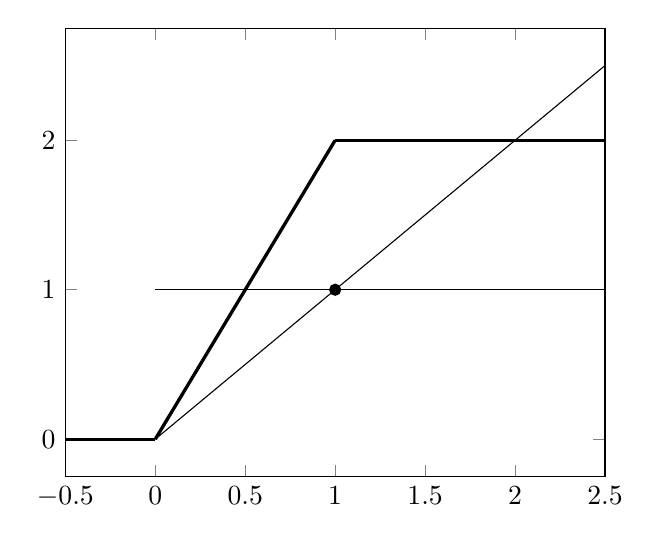
\begin{tikzpicture}
            \begin{axis}[xmin=-0.5,xmax=2.5]
                \addplot[domain=0:3]{1};
                \addplot[domain=0:3]{x};
                \addplot[domain=0:1,very thick]{2*x};
                \addplot[domain=1:3,very thick]{2};
                \addplot[domain=-1:0,very thick]{0};
                \addplot[soldot] coordinates {(1,1)};
            \end{axis}
        \end{tikzpicture}
    \end{figure}
    \FloatBarrier
    Minmod follows the bottom of the Sweby Region, Superbee follows the top of the Sweby region, and MC and Van Leer go in between.

\end{document}












